\chapter{Canonical retinal progenitor cell phenomena and their explanations}
\chaptermark{Canonical RPC phenomena and their explanations}
\label{chap:RPCreview}

\section*{Synopsis}
\textit{(1) The Stochastic Mitotic Mode Explanation (SMME) for retinal progenitor cell (RPC) function is the first computational model which claims to explain RPC behaviours throughout the life of a vertebrate, and so, retinal morphogenesis. (2) This would resolve decades of theoretical deadlock between competing explanations for RPC behaviours. (3) The majority of RPC phenomena are understood in terms of proliferative and fate specification outcomes of RPC lineages. (4) Macromolecular explanations for these outcomes are diverse, and difficult to reconcile into a harmonious explanation. (5) The SMME can be understood as an effort to find order by blurring out some pertinent explanatory details. (6) The SMME promises to clarify the macromolecular underpinnings of morphogenesis in a complex neural tissue by explaining it in terms of a stochastic molecular process.}

\section{The Stochastic Mitotic Mode Explanation (SMME)}
The work presented in \autoref{chap:SMME} examines the best-developed theory of \textit{D. rerio} retinal progenitor cell (RPC) function. The theory in question is the work of pre\"{e}minent retinal biologist William Harris' research group, referred to hereafter Stochastic Mitotic Mode Explanation (SMME). This theory purports to explain the function of zebrafish RPCs in terms of stochastic effects on mitotic mode, which specifies the mitotic state and fate propensity of offspring.

The SMME for RPC function is of fundamental theoretical and practical interest. It is a concerted effort to explain how a complex tissue like a retina can arise from a field of similar proliferating cells. In 2009, Harris coauthored a detailed review chapter, documenting the bewildering array of macromolecules and cellular processes thought to be involved in RPC function \cite{Agathocleous2009}. This enumeration contains many caveats and notes that the effects of particular macromolecules routinely differ between developmental stages, cell types, organisms, and so forth. At this time, no clear, detailed, comprehensive models of RPC function had been advanced, and the review is typified by statements like ``It is difficult to reconcile all the studies on the initiation and spread of neurogenesis in a single model."\footnote{This was in no sense a problem with Harris' understanding. A similarly high-level review coauthored by Pam Raymond \cite{Adler2008} concluded, with regard to models of photoreceptor fate specification: ``The data reviewed in the preceding sections indicate that a ‘one-size-fits-all’ model is not possible..."} It is therefore remarkable that, over the next nine years, a \hyperref[ssec:SSM]{simple stochastic model} of zebrafish RPC function invoking two named macromolecules would dominate the RPC literature.

The explanation aims to advance a simple, comprehensible, ``mind-sized" model of RPC function, which is a microcosm of the broader promise of ``Systems Biology" to make sense of the contemporary welter of conflicting datasets. By using sophisticated mathematical methods drawn from information and complexity theories, the apparent confusion will be clarified and underlying molecular mechanisms will be revealed. Given Harris' track record and pre\"{e}minence in the field, we have good reason to take seriously the possibility that the SMME has succeeded. Examining whether this is the case is our first priority. To appreciate the scope of his theoretical maneuver, and possible alternatives to it, we begin by summarising the state of the art at the time of his 2009 review (as well as relevant subsequent additions).

\section{Explanations for RPC function in 2009 and the drive to unification}
\label{sec:TheoryOptions}
Molecular biologists have sought explanations for the same remarkable features of retinal progenitor cells for decades. Animal retinas, having well-understood functions and stereotyped structures, promise tractable  targets for typical molecular biological explanations. With well defined cell types present in tightly regulated proportions and topological organisations, both theoretically-inclined molecular biologists and clinically-inclined regenerative medical practitioners have found the retina to be a useful model tissue\footnote{Indeed, if central neuroregenerative medicine is to become a clinical possibility, it seems likely that the theoretical and practical issues are most likely to be resolved in eyes before other areas of the CNS.}. The regular, easily detected order in eyes seemed to suggest a similar level of order and regularity in the macromolecular processes which underlay the formation of the tissue. Older explanations commonly suggested that RPCs are more-or-less identical and go through rigidly stereotypical macromolecular processes. It is, however, the persistently observed departures from this conception that have occupied much of our attention.

The simplest explanation for the regularity of retinal development is that any given RPC is executing the same strict ``developmental program" as its neighbours. If every progenitor produces a similar number of cells, and the progeny are specified in similar proportions, well-understood principles of cellular adhesion could give rise to the characteristic laminar organisation observed in animal retinas. However, by the 1980s, vertebrate lineage tracing experiments revealed a surprising degree of inter-lineage variability in many neural progenitor systems, not least of which was the retina. In their seminal 1987 paper, David Turner and Connie Cepko, using retroviral lineage labelling techniques, demonstrated that individual RPC lineages in rats had diverse proliferative and fate specification outcomes \cite{Turner1987}; Harris' group confirmed this result in \textit{Xenopus} the subsequent year \cite{Holt1988}, suggesting this variability was a common feature of vertebrate RPC function.

Indeed, at this point, we find fairly clear accounts of what retinal biologists took their theoretical options to be in explaining this variability. As Harris' 1988 report states:

\begin{longquote}
Changes in cell character associated with cell type diversification may be controlled in an autonomous way, reflecting either a temporal program inside the cell (Temple and Raff, 1986), the asymmetrical segregation of cytoplasmic determinants (Strome and Wood,
1983; Sulston and Horvitz, 1977), stochastic events inside the cell (Suda et al., 1984), or some combination of
these processes. Alternatively, cell type may be controlled in a nonautonomous way, as in cases in which
the extracellular environment (Doupe et al., 1985) or
cellular interactions (Ready et al., 1976) elicit or limit cell
fate. With its multiplicity of cell types, the vertebrate nervous system would seem to require the ultimate sophistication in its means of cellular determination. 
\cite{Holt1988}
\end{longquote}

It is striking, then, that Harris' review of the literature two decades later describes the situation similarly:

\begin{longquote}
Once differentiation is initiated, regulatory
mechanisms within the retina ensure that progenitors retain the capacity to undergo more
divisions, in parallel with churning out differentiated cells, and that progenitors cease dividing at variable times. There is still debate
about the extent of early programming that allows progenitors to step through a series of
stereotypical divisions and the extent of regulation from within the whole retina. The production of differentiated cells alters the retinal
environment with time...

Moreover, cells from the same clone do not all
differentiate at the same time, suggesting three
possibilities: a stochastic mechanism for the
decision to differentiate, exposure of the two
daughters to different environments, or asymmetric inheritance of determinants.
\cite{Agathocleous2009}
\end{longquote}

In the same paper, he states that the ``simple structure and accessibility of the retina make it a useful model to study cell division and differentiation, and as a result most aspects of this have been studied, from lineage tracing of progenitors, to the morphological aspects of division, to the molecular mechanisms involved." Thus, by Harris' own account, some twenty years of additional research into almost every variety of macromolecular explanation for a huge range of RPC-related phenomena had not provided any means to narrow down the possibilities he had already laid out in 1988. We still have Raff's temporal program ("early programming ... step[ping] through a series of steretypical divisions"), asymmetric segregation of cytoplasmic inheritants during mitotic events, ``stochastic" events internal to the cells, and possible ``environmental" extracellular determinants. While the number of particular macromolecules functionally implicated in proliferative, specificative, and organisational RPC phenomena had greatly expanded, this had not provided any means to differentiate between these theoretical options. This is only one example of a general phenomenon, in which enumerationist research programs, directed at producing more and more facts about macromolecular involvement in cellular phenomena, have failed to generate additional theoretical understanding \cite{Kaneko2006}. Harris' SMME therefore represents an example of a ``Systems" biological explanation, in which biologists apply the analytical and interpretative methods of the physical and mathematical sciences in an effort to resolve the problems posed by biological complexity \cite{Morange2009}.

Before proceeding to the SMME itself, let us briefly summarise the diversity of phenomena implicated in RPC function by 2009, as well as the panoply of mechanisms offered as explanations. In doing so, it will become clear what has been elided in the SMME, and what may need to be restored in any alternative modelling approach.

\section{Canonical vertebrate RPC phenomena: the RPC ``morphogenetic alphabet"}

The bulk of our knowledge of RPC behaviour stems from histological observation employing a limited number of techniques. Simple observations of mitotic figures in a variety of animals had, by the 1950s, revealed the surprising diversity of RPC proliferative phenomena across vertebrate clades. However, it was the advent of lineage tracing techniques, particularly those marking single clonal lineages in whole retinae, and the extensive use of these techniques in the 1980s-90s, that formed most of the basic body of observations that any macromolecular explanation is now called upon to account for.

Since the majority of vertebrate retinas of biomedical interest are mammalian, and these retinae are fully formed in an early developmental period, RPC behaviour has been best-studied in an embryonic and early developmental context. Here, vertebrate RPCs are derived from the eye field population of the early neural plate and later neural tube. This population is separated into left and right eye primordia, which in turn pouch outwards toward the ectoderm, and, in conjunction with the lens placode (itself induced from the ectoderm), form the optic vesicle. The primitive eye is formed when this vesicle completes a complex morphological folding process, resulting in the cup-shaped structure of the retina \cite{Cavodeassi2018}. During this process, the cells of the neural retina are differentiated from the overlying retinal pigmented epithelium (RPE). Sometime after the formation of the retinal cup, RPCs begin to exit the cell cycle and are specified as retinal neurons. Studies of this early period revealed numerous difficult-to-explain features of RPC behaviour. Following Larsen's observation that tissue form is attributable to only six behaviours \cite{Larsen1992}, which she describes as the ``morphogenetic alphabet", I have categorised RPC phenomena as relating to proliferation, fate specification, migration, growth, death, and extracellular matrix formation. Since the vast majority of reported phenomena fall under the first two categories, proliferation and specification, these are given separate sections below, while those belonging to the last four are described collectively.

\subsection{Proliferative phenomena}

Clonal lineage tracing experiments reliably find that vertebrate RPCs give rise to highly variable numbers of offspring over the collective ``lifetime'' of the lineage. The most dramatic of these findings demonstrate that rat RPC lineage sizes vary across two orders of magnitude in vivo, from 1 to over 200 \cite{Turner1990}. While at least some of this variability must be related to differential integration of lineage markers into ``older" (giving fewer offspring) and ``newer" (giving more) RPCs, vertebrate RPC lineages nevertheless differ widely in their fecundity. The physical organisation of these clones is complex; as detailed below, RPC progeny may appear in any of the 3 retinal layers in a wide variety of specified fate combinations, and may engage in short-range migrations to appropriate positions for their specified fates. Most clonal lineages are ``extinguished"; that is, after some time, all of its members have become postmitotic. However, it has long been noted that not all cells produced by RPCs are strictly postmitotic neurons; specified M{\"u}ller glia retain the ability to reenter the cell cycle in response to stimuli (normally, retinal damage) \cite{Dyer2000,Fischer2003a}, and peripheral CMZ RPCs remain proliferative in those vertebrates whose eyes grow beyond early development (notably in frogs and fish, while the chick retina has a CMZ of more limited output \cite{Fischer2000}). Therefore, some clonal lineages may be organised into clumps associated with M{\"u}ller responses, while others in frogs and fish may continue to be ``plated out" in a more-or-less linear manner at the retinal periphery for as long as the lineage ``lives" \cite{Centanin2011}. This ongoing RPC contribution to peripheral neurogenesis has long been recognised, so that by 1954 we find the following statement introducing a study of unusual mitoses in the retina of a deepsea fish: 

\begin{longquote}
  It is conventional\footnote{Unfortunately, I am unable to locate the source of this convention, likely due to the poor preservation of many of these older reports. That this required no citation in 1954 suggests the original observations of CMZ proliferation may be in the early 20th century.} to hold that the growth of the vertebrate retina is only possible due to the presence, in this tissue, of a peripheral germinal zone. In this region, young elements actively multiply, and, by subsequent differentiation, give rise to the diverse nervous and sensory constituents of the retina.
  \cite{Vilter1954}
  
  [author's translation from the French]
\end{longquote}

Despite this, the proliferating RPCs in this ``peripheral germinal zone" (also known as the ``ciliary marginal zone", or CMZ, for its proximity to the retinal ciliary body) have not received the same level of attention as those associated with the central retina. As a consequence, these RPCs are generally treated as though they are a type of ``frozen" progenitor population, recapitulating spatially, along the peripheral-central axis, the process which RPCs in the central retina undergo in a time-dependent fashion \cite{Harris1998}.

The length of the RPC cell cycle is of considerable interest, since the evolution of this parameter in time, in conjunction with the RPC population size (the number of cells specified in the eye field), determines the eventual size of differentiated retinal neural population, and therefore the retina. RPC cell cycle length is usually inferred from clonal lineage size, although it has also been assayed directly in cumulative thymidine analogue labelling experiments \cite{Alexiades1996}. Vertebrate RPCs undergo a period of relative quiescence, in which the cell cycle lengthens, before the neural retina begins to be specified (in zebrafish, this period is ~16-24 hpf). The cell cycle shortens as RPCs begin to exit the cell cycle \cite{Harris1991,Li2000}. After the central retina is specified, the RPC cell cycle again lengthens, and is presumed to continue to slow until RPCs have completed specifying\footnote{This presumption is demonstrably incorrect in the \textit{D. rerio} eye, see \autoref{sec:sliceGMC} for a more plausible model of cell cycle dynamics in this organism.}.

Finally, the orientation of the RPC division plane in mitosis is also  implicated in retinal organisation. The orientation of divisions is associated with the both proliferation and fate specification of RPC progeny. For instance, interfering with spindle orientation in the developing rat retina, such that more RPC divisions occur parallel to the neuroepithelial plane (rather than along the apico-basal axis) results in more proliferative and fewer postmitotic, specified progeny \cite{Zigman2005}. That said, it seems that whatever effects are attributed to mitotic orientation are likely species-specific, as zebrafish RPCs display a different pattern of axis orientation, dividing mainly in the epithelial plane \cite{Das2003}.

\subsection{Fate specification phenomena}

Offspring of vertebrate RPC lineages may enter any of the three cellular layers of the retina. Moreover, single lineages can include any possible combination of cell fates, so that RPCs cannot be readily divided into ``types" on the basis of lineage fate outcomes \cite{Holt1988,Turner1990,Wetts1988}. While some progenitors have propensities to generate similar cell types, these relations seem species-specific, and may not define separate progenitor pools \cite{Adler2008}. In general, then, RPCs are taken to be multipotent with respect to the neural retina- all of the cell types\footnote{The ``cell type" concept is unusually well-defined in the retina, as there are an abundance of distinct morphological and molecular features which differentiate numerous subtypes of the seven general types of retinal neuron.} of the differentiated retina are derived from similar RPC lineages. Little about this picture has changed since its initial development, using a variety of lineage tracers (including retroviruses, thymidine analogues, and injectable dyes) and histochemical markers to supplement morphological identification of specified neurons. In particular, sophisticated modern live imaging experiments in zebrafish (many pioneered by Harris), have broadly confirmed the findings of the 80s and 90s in mammalian fixed specimens, explants, and live animals \cite{Boije2015}.

\label{Raff}
Of particular note are the observations of the Raff group \cite{Watanabe1990,Cayouette2003}, who demonstrated that dissociated rat RPCs, cultured at clonal density, took on morphological and histochemical features associated with different specified neural types in similar numbers and proportions, and on a similar schedule, to same-aged RPCs cultured in retinal explants. These results dramatically suggested that both the proliferative and fate specification behaviour of RPCs depends less on intercellular contact, and the complex signalling environment of the developing retina, than on factors intrinsic to the RPCs themselves. These studies contain the essential germ of Harris' eventual commitment to SSM explanations, purporting as they do to ``test the relative importance of cell-intrinsic mechanisms and extracellular signals in cell fate choice", and providing convincing evidence for the preponderant importance of the purported cell-intrinsic mechanisms.

\begin{figure}[!h]
  \makebox[\textwidth][c]{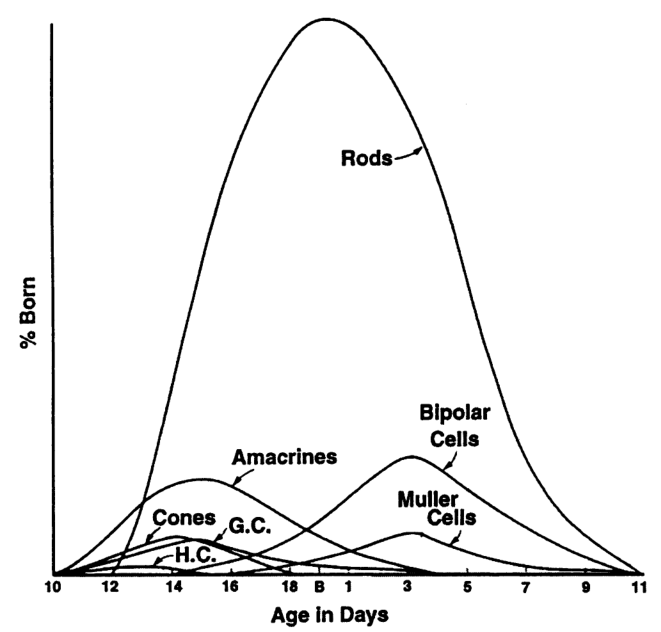
\includegraphics[width=.7\textwidth]{cepko0.png}}
  \caption{{\bf Histogenetic birth order of retinal neurons}}
  Adapted from \cite{Young1985} by \cite{Cepko1996}. G.C., Ganglion Cells; H.C., Horizontal Cells. Data from embryonic and perinatal mouse eyes.
  \label{horder}
\end{figure}

In spite of the apparent ability of RPCs to produce offspring specified to any of the possible neural cell fates, at any time during their lineage history\footnote{Even in papers arguing for a strict, linear sequence of specificative outcomes in all RPC lineages, the actual data show RPCs occasionally giving rise to ``late-born" photoreceptors subsequent to their first division \cite{Wong2009}, giving lie to the notion that the process is particularly strict.}, vertebrate retinal development displays a temporal ordering, such that in any particular location, retinal ganglion cells (RGCs) tend to be produced first, followed by the other cell types in what has been described as an overlapping ``histogenetic order", pictured in Figure \ref{horder}. As noted above, RPCs also exit the cell cycle in a spatiotemporally defined order (from central to peripheral over time), and specification follows the same pattern\footnote{In many studies, cell cycle exit is conflated with specification such that evidence of the former is taken as evidence of the latter. There are, however, reasons to believe cell cycle exit and specification are not the same process, discussed below.}. This naturally gave rise to questions about the origin of the ``overlap" observed in the sequential production of various cell types; conceptually, this overlap could be produced by identical RPCs executing identical rigid specification programs if they begin to execute it along the spatiotemporal gradient noted above, as originally suggested by Cepko et al. \cite{Cepko1996}. However, it is impossible to reconcile this notion with more recent results from Harris' \textit{in vivo} zebrafish lineage tracing studies \cite{Das2003,He2012,Boije2015}, which confirm mammalian cell culture work in demonstrating that vertebrate RPC lineages do not execute similar specificative programs. More recent articulations of Cepko's concept of linear specification programs incorporate variable sub-programs to account for this \cite{Cepko2014}.

\subsection{Other morphogenetic phenomena}
The outcomes of RPC proliferation and lineage commitment are often taken as sufficient explanation for the formation of the neural retina. Indeed, after the eye cup has been formed (prior to the specification of any neurons), RPCs are, in effect, already ``in place". Therefore, there are few documented RPC phenomena outside of the ``proliferation" and ``specification" categories of the morphogenetic alphabet \cite{Larsen1992}, which ennumerates the cellular processes contributing to tissue form and structure. RPCs do not seem inclined to migrate long distances , they seem not to generate much in the way of extracellular material\footnote{The formation of a laminin-rich basement membrane seems to be necessary for optic vesicle formation \cite{Ivanovitch2013}, but it is not clear that RPCs produce this. ECM function in eye formation remains under-studied.}, and, in non-pathological conditions, they are rarely seen to die. Still, there are a number of phenomena which appear to be important for proper retinal organisation that fall into these other ``alphabet" categories.

The most notable of these is interkinetic nuclear migration (INM), in which RPC nuclei move back and forth between the apical and basal surfaces of the retina. Common in many neural tissues, INM affects both proliferation and fate specification, but is dissociable from them- both cell cycle and specification proceed (albeit in a precocious manner) when INM is disrupted \cite{Murciano2002}. The apical retinal surface provides a microenvironment which appears to be required for RPC mitosis to occur\footnote{Nonapical divisions do occur, notably in specified, but proliferative cells \cite{Godinho2007}. The extent to which RPCs depend on the apical surface may depend on how ``RPC" is defined. In general, RPCs are no longer considered as such when they acquire characters associated with differentiated neurons (cell type markers, morphological traits, etc.), although it is clear that the acquisition of these characters does not necessarily imply that the cell is postmitotic. Any complete explanation of how RPCs give rise to the structure of the eye must also consider these nonapical divisions.}, and INM seems to consist of a directed, probably actomyosin-mediated movement to the apical surface, followed by an undirected ``random walk" away from the apical surface and hence toward the basal retina \cite{Norden2009}. This ``random walk" may arise from displacements due to the directed INM of neighbouring progenitors \cite{Azizi2020}. More committed RPCs also appear to actively migrate to positions appropriate for the specified cell type \cite{Chow2015,Icha2016}, although it is unclear if this short-range migration is caused by INM undergone by more actively proliferating progenitors. It seems likely that these short-range migrations of more specified cells are especially significant in the early retina, before the neural plexiform layers (consisting of axons and other neural processes) have begun to divide the cellular layers into bounded compartments.

Notable gaps in the study of the RPC ``morphogenetic alphabet'' include the regulation of cell size and growth, and potential roles for cell death, both of which have received little attention.  Cell size and growth are closely linked to proliferative behaviour in yeast \cite{Yang2011}, and studies have been conducted in Schwann cells and oligodendrocytes \cite{Conlon2001}, but related effects in RPCs have not been elucidated. This may be a significant oversight, given the requirement for RPCs to continuously grow during their proliferative lifespan. Cell death does not seem to play the same ``pruning" role for RPCs that it often does in other neural tissues, and observed rates of cell death in normal RPC populations are very low, so few studies have been conducted.

\section{Macromolecular mechanistic explanations for RPC phenomena}

Having surveyed the cellular phenomena pertaining to RPC function in retinal development, we proceed to a selection of the many macromolecular mechanistic explanations (MEx) \cite{Fagan2012} that have been offered to explain them. Unsurprisingly, given the field's focus on the early events of eye development, these MEx are mainly targeted at this period. Thus, the majority explain tissue-level phenomena like the initial ``wave" of cell cycle exit and specification, without necessarily seeking a global explanation for RPC behaviour irrespective of context, so it is unknown how many of these might pertain to ongoing peripheral neurogenesis or other, adult neurogenic phenomena like those exhibited by M{\"u}ller glia. That said, we now turn to examine some of the best-developed of these explanations.

\subsection{Transcription factor networks}

Perhaps the most notable MEx offered to explain RPC specification and development is the eye field transcription factor network, or EFTFN. The roots of this explanation are found in the Pax6 ``master gene" explanation popularised in the 1990s \cite{Gehring1996}. This explanation revolved around the apparently universal involvement of Pax6 gene products in eye formation in model organisms, and the promiscuous inter-species effects of Pax6 (with mouse RNA able to induce ectopic formation of eye structures in \textit{Drosophila} imaginal discs, for instance \cite{Halder1995}), so that it appeared to be a highly conserved genetic ``switch" for eye development.

Importantly, this explanation purported to resolve what Darwin regarded as a serious problem for his theory, the apparent implausibility of the gradual evolution of eyes (and other ``organs of extreme perfection") from some primitive ancestral structure \cite[p.143-4]{Darwin1888}. In particular, Pax6 suggested to some theorists an alternative to the surprising hypothesis of Mayr and Salvini-Plawen, that differences in eye structure and function across clades indicate the independent appearance of eyes in more than 40 clades \cite{v.Salvini-Plawen1977}. Pax6 thus provided a molecular pointer to a potential common ancestor for all animal eyes \cite{Erclik2009}.

Subsequent investigations revealed that vertebrate Pax6 is a conserved member of a complex network of cross-activating and inhibiting transcription factors, including Pax6, Rx1, Six3, Six6, Lhx2, ET, and Tll \cite{Zuber2003}. Members of this network tend to promote proliferation and suppress markers of differentiated neurons, and their loss commonly results in the failure to form the eye field at all \cite{Agathocleous2009}. The expansion of this explanation to include other TFs in a network revealed significant differences between species \cite{Wagner2007}- while the role of Pax6 is conserved between \textit{Drosophila} and vertebrates, the roles of other members of the EFTFN are not. Moreover, the universality of Pax6 was only apparent, and not real, as there are bilaterian eyes whose development is Pax6 independent (including in \textit{Platynereis, Branchiostoma}, and planarians) \cite{Kozmik2008}. This highlighted the great difficulty in connecting morphological characters such as those observed by Mayr with a genetic basis- it is simply not clear that Pax6 conservation points to a common ancestor for all eyes, or even all photoreceptive neurons\footnote{Indeed, the relevant ``unit" of homology for evolutionary explanations for eyes remains contested, with some arguing for the cell itself over any particular set of gene sequences \cite{Erclik2009}}. Moreover, expansion of the monocausal ``master gene" explanation, to include a network of TFs with broad gene regulatory effects, highlighted the problems of complexity in offering MEx for RPC function. The components of this network interact in complex, context-dependent ways. While the EFTFN as a whole is taken to promote RPC proliferation and to delay specification\footnote{This is sometimes referred to as ``promoting RPC fate", since RPCs are taken to be those cells which proliferate but do not yet display markers of specification. Since it is, by now, widely recognised that cells that appear to be well-specified may remain in cell cycle \cite{Godinho2007,Engerer2017} this terminology should probably be jettisoned.}, its components have also been held responsible for the specification of particular classes of differentiated neurons, and remain expressed in those postmitotic cells. Notably, Pax6 is implicated in the expression of bHLH TFs required to specify multiple classes of retinal neuron \cite{Marquardt2001}, and is known to directly activate Ath5, necessary for RGC specification \cite{Willardsen2009}. The EFTFN has thus been offered as an explanation for the maintenance of the multipotent, proliferative RPC state, but how this network is disassembled, and its components repurposed to promote specification, remains obscure.

The EFTFN is not the only transcription factor network offered as a MEx for RPC function. Another well-developed explanation involves Chx10 (aka vsx2), a transcription factor important for normal proliferation of RPCs, its loss causing microopthalmia in the mouse \cite{Burmeister1996}. Chx10 was subsequently found to repress Mitf, involved in RPE specification, and hence to promote neural retinal fates over pigmented epithelial ones \cite{Horsford2004}; in the absence of Chx10 the early eye cup does not stratify properly between apical pigmented cells and the neural retina. Much like the multifunctional EFTFN components, Chx10/vsx2 has also been implicated in the specification of particular neural fates, notably bipolar neurons \cite{Burmeister1996} and the regulation of Vsx1 (a paralogue of Chx10), Foxn4, and Ath5, associated with specification of subpopulations of bipolar cells, horizontal and amacrine cells, and RGCs and PRs, respectively \cite{Clark2008,Vitorino2009}.

Clear hypotheses advocating for particular relationships between different TF-centric explanations are rarely stated. It is tempting simply to arrange them in some kind of ``developmental order", perhaps with the Chx10-Mitf network ``downstream" of the EFTFN. That this would be facile is evident from the changing roles of these transcription factors, depending on developmental and cellular context. To date, no unifying framework has been applied. Obvious candidates include the ``developmental gene regulatory network" concept \cite{Li2009}, a type of cybernetic explanation which assembles genes into feedback networks. Given the popularity of this type of explanation, it is worth noting that no one has yet had any success in offering one for RPC function.

These transcription factor network MEx frequently incorporate extracellular signals (often as an explanation for the appearance or ``set-up" of the TF network), and it is generally recognised that these signals have a profound influence on these networks, and on RPC behaviour generally. We therefore turn to explanations invoking these signalling mechanisms.

\subsection{Intercellular signalling networks}

Virtually every developmentally significant class of signal had been implicated in RPC function by 2009 \cite{Agathocleous2009}. These include BMP, CNTF, FGF, Glucagon, Hedgehog, IGF, Notch, TGF$\alpha$, TGF$\beta$, VEGF, wnt, and a host of neurotransmitters. This diversity of signalling pathways has proved to be a formidable problem for integrated explanations, since almost all of these pathways converge on the same two cellular outcomes in RPCs, that is, proliferation and specification. Thus, most signalling MEx for RPC function elide the majority of other signals which are known, or thought, to affect the same processes. That said, let us explore a few of the more detailed signalling explanations.

In developmental terms, the first phenomenon requiring explanation is the appearance of the eye field to begin with- what is it that accounts for the differentiation of RPCs from the rest of the anterior neural plate and tube? Wnt signalling MEx have been offered to explain the appearance of the \textit{Xenopus} eye field. Fz3 signalling seems to promote expression of eye field transcription factors (see below) \cite{Rasmussen2001}, while an unspecified non-canonical interaction between Wnt11 and Fz5 inhibits canonical $\beta$-catenin signalling through Wnt8b/Fz8a, which would otherwise promote prospective anterior forebrain fates \cite{Cavodeassi2005}. Inhibition of FGFR2 signalling, and activation of ephrinB1 signalling have also been implicated in early \textit{Xenopus} eye field cell movements \cite{Moore2004}. Subsequent experiments determined that the xenopus ADP signalling through the P2Y1 receptor directly activates the EFTFN \cite{Masse2007}, described above. More recent experiments in zebrafish suggest that precocious acquisition of neuroepithelial apicobasal polarity, probably driven by interactions with a Laminin1 basement membrane, distinguishes the early eye field \cite{Ivanovitch2013}.

Subsequent to the appearance of eye field RPCs and their rearrangement into the optic cup, the apparent central-to-peripheral ``wave" of RPC exit from cell cycle and specification of early RGCs \cite{Hu1999}, has had detailed MEx advanced to explain it. In both zebrafish and chick retina, FGF3 and FGF8, originating from the optic stalk, initiate this early cell cycle exit and specification \cite{Martinez-Morales2005}, while inhibiting FGF signalling prevents this from occurring, and ectopic expression of FGF can cause it to occur inappropriately. The progression of this ``wave" of cell cycle exit and specification has been separately explained, by Sonic Hedgehog (Shh) signalling from the newly specified RPCs inducing cell cycle exit and specification in adjacent cells \cite{Neumann2000}. This process is dependent on, and downstream of, the above-mentioned FGF induction \cite{Martinez-Morales2005}. The role of Hh signalling has been challenged on the basis that Hh inhibition in subsequent experiments did not display the same effect size \cite{Stenkamp2003}, and that its effects on Ath5 expression, required for RGC specification, are ambiguous \cite{Agathocleous2009}. More recent MEx have suggested that Hh signals may decrease the length of the cell cycle, resulting in increased proliferation and earlier cell cycle exit and specification \cite{Locker2006, Agathocleous2007}.

A well-developed ``local" signalling MEx invokes the classic Notch/Delta lateral inhibition model, with small fluctuations in Notch/Delta activity giving rise to a positive feedback response that differentiates neighbouring cells. Cells which have high Delta expression tend to be specified as retinal neurons, while those with high Notch tend to remain proliferative, either as RPCs or M{\"u}ller glia \cite{Dorsky1995,Dorsky1997}. More recent results implicate asymmetric inheritance of Sara-positive endosomes in the partitioning of this signal \cite{Nerli2020}.Such a mechanism could regulate the activity of both early, central RPCs, as well as peripheral RPCs, and may contribute to inter-RPC variability. These differences between RPCs located in different parts of the developing retina have been of significant interest, and it is worth briefly examining patterning MEx that may also explain spatial differentiation between RPCs.

\subsection{Patterning mechanisms}

Among the most interesting features of RPCs is that they reliably give rise to specified neurons, in particular RGCs, that seem to ``know where they are" in the retina, enabling them to wire their axons in correct retinotopic order in the superior colliculus (SC) or optic tectum (OT). The most developed MEx explaining this refer to gradients of EphA and EphB receptors expressed in RGCs, and their respective ephrin ligands expressed in the SC or OT. In the retinal RGC population, an increasing nasotemporal gradient of EphA is paired with an increasing dorsoventral gradient of EphB. A corresponding increasing rostrocaudal gradient of ephrin-A is paired with an increasing lateromedial gradient of ephrin B in the SC/OT. 
This allows for a two-axis encoding of an RGCs' position in the retina \cite{Tsigankov2006}. As the RGCs' axon pathfinding depends on repulsive effects mediated by Eph receptors, this code is sufficient to allow correct wiring of even single RGCs \cite{Gosse2008}. The action of Gdf6a seems to establish this code in RPCs themselves, prior to specification \cite{French2009}.

Indeed, there are numerous similar observations of expression gradients that create spatial differences between RPCs themselves. Most relevant to the proliferation dynamics highlighted in this chapter is the observation that, in \textit{Xenopus} eyes, a decreasing dorsoventral gradient of type III deiodinase renders the cells of the dorsal CMZ refractory to thyroid hormone (as the deiodinase inactivates TH) \cite{Marsh-Armstrong1999}. The effect of this is to set up a differential response to TH in post-metamorphic RPCs, so that the ventral population selectively expands in response to TH \cite{Beach1979}. 

These patterning mechanisms are of particular interest here, in large part because they clearly establish that the RPC population is heterogenous, both with respect to proliferative and specificative behaviours, and perhaps others as well. This is of critical importance for any modelling effort, as virtually all \hyperref[ssec:SSM]{mathematical models used by stem cell biologists} (and those used to justify Harris' SMME) assume, at least initially, homogenous populations of stem or progenitor cells. Since RPCs do not meet this condition, special care is needed to use these models.

\subsection{Chromatin dynamics}

In recent years, the great importance of chromatin conformation in RPC proliferation and specification has become more clear. Indeed, chromatin dynamics are now widely invoked in explaining stem and progenitor cell behaviour, and suggested as a target for cell reprogramming \cite{Kondo2006,Tee2014}. In RPCs, detailed accounts of three-dimensional chromatin dynamics have yet to appear. However, a number of studies point to the importance of chromatin state in informing the overall cellular state. In particular, histone deacetylation seems to be important for RPC specification, as the loss of histone deacetylase 1 (HDAC1) in zebrafish results in overproliferation and decreased specification, and correlated increases in Wnt and Notch activity \cite{Yamaguchi2005}. In mouse retinal explants, decreased proliferation and specification result from  pharmacological inhibition of HDAC \cite{Chen2007}. Additionally, the chromatin remodelling complex SWI/SNF has repeatedly been implicated in RPC function. Notably, one particular component of this complex seems to be particularly associated with vertebrate RPCs (BAF60c, an accessory subunit) \cite{Lamba2008}. A switch to other subunits seems to be necessary for specification \cite{Lessard2007}. Details regarding the subunits involved in specification and their downstream effects are complex and context dependent, much like the signalling pathways mentioned above.

\section{A unified theory of RPC function? ``Blurring" to order}

From the foregoing discussion, we can see the theoretical conundrum. Macromolecular explanations for RPC behaviours, like those throughout the molecular biological tradition, have generally been built outwards from particular transcription factors, receptors, etc. The result is an archipelago of MEx, at best connected by tenuous speculation, and in most cases, without any known means to form an integrated model. Furthermore, the degree of complexity and context-dependence evident from the literature might seem to preclude such a model. As we have seen, multiple reviews found that the evidence did not allow for clear discrimination between logically distinct types of mechanisms for producing the observed variability in RPC lineage outcomes.

In this situation, there were two theoretical options. The first is simply to ``crank the handle"- to generate more and more facts describing the difference particular molecules make to RPC outcomes in dozens of relevant contexts, piling up exceptions and idiosyncracies, in the hope that doing so will eventually bridge the explanatory ``islands" of the MEx archipelago. This has been referred as the enumerationist approach by Kaneko, who ably explains why it is doomed to failure \cite[pp.31-32]{Kaneko2006}. The second option, the one actually chosen by Harris, is more theoretically sophisticated. As Nicholas Rescher has noted regarding in-principle limits to scientific knowledge, the phenomenal universe has infinite descriptive complexity- one can always add more detail to a description of some phenomenon, and no such description is ever complete \cite[p.22-9]{Rescher2000}. Moreover, ``even as the introduction of greater detail can dissolve order, so the neglect of detail can generate it." \cite[p.62]{Rescher2000} As Rescher goes on to comment:

\begin{longquote}
[W]e realize that in making the shift to greater detail we may well lose information that was, in its own way, adequate enough ... information at the grosser level may well be lost when we shift to the more sophisticated level of greater fine-grained detail. The 'advance' achieved in the wake of 'superior' knowledge can be - and often is - purchased only at a substantial cognitive loss.

...

It is tempting on first thought to accept the idea that we secure more - and indeed more useful and more reliable - information by examining matters in greater precision and detail. And this is often so. But the reality is that this is not necessarily the case. It is entirely possible that the sort of information we need or want is available at our 'natural' level of operation but comes to be dissolved in the wake of greater sophistication.
\cite[p.65-6]{Rescher2000}
\end{longquote}

Rescher's greater point is that ``blurring" detail, at levels below the phenomenal one under consideration (for RPCs, generally, the cell or lineage), may be necessary to produce an ordered explanation that is useful for some objective. Given the number of overlapping and contradictory MEx for RPC behaviour, we have the situation Rescher is describing- more sophistication, and more detail, has dissolved order, not revealed it\footnote{At least part of this problem is likely related to the fact that the majority of biomedical findings cannot be replicated \cite{Ioannidis2005}. The finding, mentioned above, that Shh effect sizes on RPC function were not as large as initially reported when subsequently investigated, is typical and symptomatic of this replication problem. ``Blurring" may therefore be necessary not only because of fundamental epistemic limits, but also because it is often difficult to distinguish bona fide results and explanations from spurious ones.}. The inability to assemble an unified explanation for RPC function has left us without fundamental understanding of how highly ordered neural tissues like eyes are generated from composites of units with highly variable, temporally and spatially ordered outcomes like RPC lineages. As this is a common feature of vertebrate neurogenesis more generally, this leaves us without the ability to produce complete models of neurodevelopmental processes in many species. Moreover, in the absence of a clear framework for comparing the explanatory power of the diverse array of MEx so far advanced, practical contributions of clinical relevance have been scanty and tentative, with RPC transplantation, and more recently, gene therapies taking little note of complex MEx for RPC function \cite{Coles2004,Gaillard2007,Yao2018}.

In a situation of this kind, this type of ``blurring" is required, and it seems that by cutting down to the simplest possible explanation, the SMME hopes to bring into view order that was previously obscured by detail. There is, of course, a significant danger here: how does one decide what is ``blurred out" and what remains? We can easily understand how a practicioner's biases could lead to a sort of relativism, where the ``blurring" makes apparent a spurious order that conforms to these biases rather than to reality as such. With this in mind, let us survey the general thrust of the SMME, before proceeding to examine it in detail, in \autoref{chap:SMME}.

\section{Explanatory Strategy and Intent of the SMME}
\label{sec:SMMEexplanatorystrat}
As we have seen in \autoref{sec:TheoryOptions}, Harris' long-held understanding of the explanatory options for RPC function divides them into four broad categories:

\begin{enumerate}
\item A linear algorithmic ``program" of proliferation and specification
\item Asymmetric segregation of specificative determinants
\item ``Stochastic processes" internal to the cells
\item Influences of extracellular factors
\end{enumerate}

Harris' sophisticated discussions of RPC MEx rarely treat these categories as exclusive, and concede that good explanations for RPC behaviour may involve phenomena from more than one of them. Indeed, the SMME necessarily contains elements that Harris concedes are ``linear" and ``deterministic" \cite{He2012}. Still, his overall strategy for the SMME is, first, to substantiate the predominant influence of one of these categories of phenomena (that is, category 3, internal stochastic processes or effects), and subsequently to specify an actual macromolecular system that could plausibly be such an ``internal stochastic process". These two theoretical maneuvers, while tightly linked, serve different purposes within Harris' overall explanatory framework, which must be examined separately.

The SMME for zebrafish RPC function has been developed across three separate papers \cite{He2012,Boije2015,Wan2016}. Each builds on the earlier publications, collectively purporting to explain the behaviour of RPCs wherever, and whenever, they may be found in the zebrafish eye. The underlying model is originally derived from an earlier paper pertaining to rat RPCs \cite{Gomes2011}. He et al. \cite{He2012} and Wan et al. \cite{Wan2016} use essentially the same model and make up the substance of the first of these two maneuvers. Boije et al. \cite{Boije2015} substantially modifies this model, specifying the activity of two known transcription facts (Ath5 and Ptf1a) as the model's biological referents. This paper constitutes the second theoretical thrust.

The first maneuver intends to support the contention that zebrafish RPCs are equipotent progenitors with variable lineage outcomes that depend on independent ``stochastic" processes within each of these cells. This is to be provided by demonstrating that a \hyperref[SSM]{Simple Stochastic Model} (SSM) of an RPC, numerically simulated many times by \hyperref[MonteCarlo]{Monte Carlo} methods to represent a population of RPCs, produces similar outcomes to populations of RPCs in vivo. This explanatory strategy is common in the stem cell literature, the original example having been published in 1964 by Till, McCulloch, and Siminovitch \cite{Till1964}. The SMME therefore represents an example of a traditional scientific logic- an explanatory pattern deployed by stem cell biologists in diverse contexts, and widely accepted because of its ongoing use in the literature, although with varying interpretations.

The success of this first maneuver thus depends on two outcomes. Firstly, the output of the SSM should accurately reflect the observed proliferative and specificative outcomes of zebrafish RPC lineages, giving weight to Harris' claim that it "provides a complete quantitative description of the generation of a CNS structure in a vertebrate in vivo" \cite{He2012}\footnote{This claim is somewhat extravagant; the SSM, by definition, includes no spatial information, so it is unclear how one could be a ``complete description" of any spatially organised structure. Still, it can be complete with regard to cell population numbers.} Secondly, the internal structure of the SSM should provide good reason to believe that one of the stochastic options is a better explanation for RPC lineage outcomes than those identified by the other three categories of theoretical options ennumerated above.

The second theoretical maneuver is the specification of particular biological referents for entities in the model. This offers an opportunity to move beyond a purely conceptual argument about the kind of process that might produce variable RPC lineage outcomes, and to begin the work of explaining how the behaviour of a particular macromolecular system constitutes such a process, so that empirically verifiable hypotheses may be generated. The success of this maneuver depends on the biological plausibility of the identification between model structure and the biological function of transcription factors, Ath5 and Ptf1a, that the model names. A good SSM-based explanation would point the way for further research by identifying \textit{how} so-called "stochastic processes" in RPCs might function, and make some predictions about this. With that said, let us turn to the SMME and determine how well these manuevers have succeeded.